\documentclass[border=0.8ex,svgnames,tikz]{standalone}
\usepackage{amsmath,mathtools}
\usepackage{fontspec}
\setmainfont{Source Serif 4}
\setsansfont{Source Sans 3}
\setmonofont{Source Code Pro}

\usetikzlibrary{calc,chains}

\begin{document}
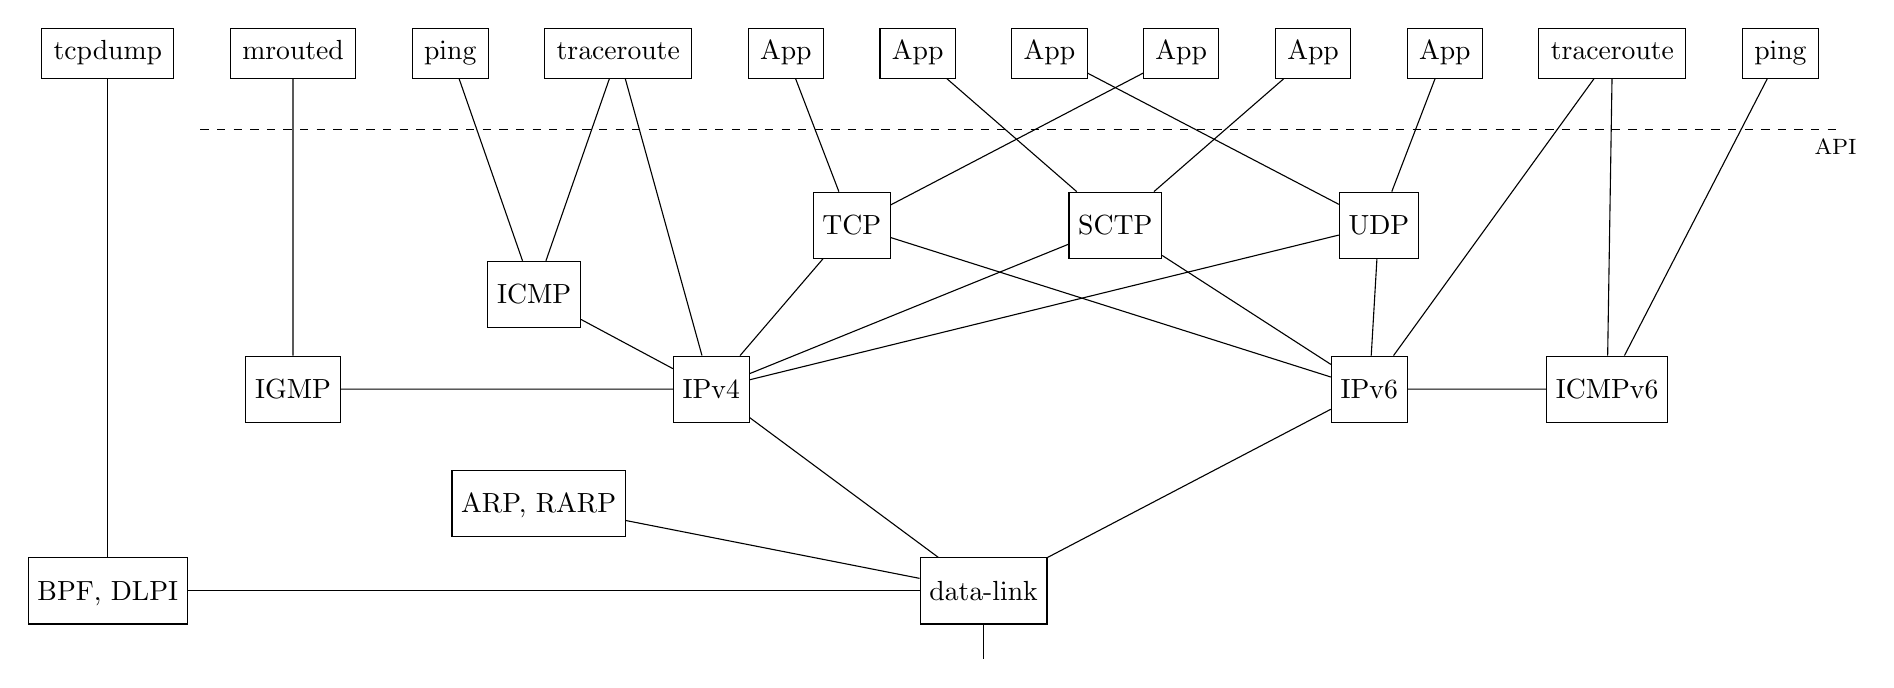
\begin{tikzpicture}
  \begin{scope}[
    every node/.style={
      draw,
      on chain,
      inner sep=1ex,
      align=center,
      text height=1.6ex,
      text depth=0.6ex,
    },
    node distance=2em,
    start chain=going mid right,
    ]
    \node (user-tcpdump)       {tcpdump};
    \node (user-mrouted)       {mrouted};
    \node (user-ping-v4)       {ping};
    \node (user-traceroute-v4) {traceroute};
    \node (user-app-tcp-v4)    {App};
    \node (user-app-sctp-v4)   {App};
    \node (user-app-udp-v4)    {App};
    \node (user-app-tcp-v6)    {App};
    \node (user-app-sctp-v6)   {App};
    \node (user-app-udp-v6)    {App};
    \node (user-traceroute-v6) {traceroute};
    \node (user-ping-v6)       {ping};
  \end{scope}
  \begin{scope}[
    every node/.style={
      draw,
      align=center,
      text height=2.8ex,
      text depth=1.2ex,
      minimum height=4ex,
    },
    ]
    \node[below=5em of $(user-app-tcp-v4)!0.5!(user-app-sctp-v4)$]
    (tcp) {TCP};
    \node[below=5em of $(user-app-udp-v4)!0.5!(user-app-tcp-v6)$]
    (sctp) {SCTP};
    \node[below=5em of $(user-app-sctp-v6)!0.5!(user-app-udp-v6)$] (udp) {UDP};
    \node[below=10em of user-mrouted] (igmp)   {IGMP};
    \node[right=12em of igmp]         (ipv4)   {IPv4};
    \node[right=21em of ipv4]         (ipv6)   {IPv6};
    \node[right=5em of ipv6]          (icmpv6) {ICMPv6};
    \node[below=7.5em of $(user-ping-v4)!0.5!(user-traceroute-v4)$] (icmpv4) {ICMP};
    \node[below left=2.4em of ipv4]     (arp)    {ARP, RARP};
    \node[below=12em of $(tcp)!0.5!(sctp)$] (datalink) {data-link};
    \node (bpf) at (user-tcpdump |- datalink)         {BPF, DLPI};
  \end{scope}
  \coordinate[below=1.25em of datalink] (out);
  \coordinate[below=2.75em of $(user-tcpdump.center)!0.5!(user-mrouted.center)$]
  (API-line-begin);
  \coordinate[below right=2.75em and 0.6em of user-ping-v6.east] (API-line-end);
  \begin{scope}[every path/.style={draw}]
    \path (user-tcpdump) -- (bpf) -- (datalink) -- (out);
    \path (user-mrouted) -- (igmp) -- (ipv4) -- (datalink);
    \path (user-ping-v4) -- (icmpv4) -- (ipv4);
    \path (user-traceroute-v4) -- (icmpv4);
    \path (user-traceroute-v4) -- (ipv4);
    \path (arp) -- (datalink);
    \path (user-app-tcp-v4) -- (tcp) -- (ipv4);
    \path (user-app-sctp-v4) -- (sctp) -- (ipv4);
    \path (user-app-udp-v4) -- (udp) -- (ipv4);
    \path (user-app-tcp-v6) -- (tcp) -- (ipv6);
    \path (user-app-sctp-v6) -- (sctp) -- (ipv6);
    \path (user-app-udp-v6) -- (udp) -- (ipv6);
    \path (user-traceroute-v6) -- (ipv6);
    \path (user-traceroute-v6) -- (icmpv6);
    \path (user-ping-v6) -- (icmpv6) -- (ipv6) -- (datalink);
    \path[draw,dashed] (API-line-begin) -- (API-line-end) node[below]{\footnotesize API};
  \end{scope}
\end{tikzpicture}
\end{document}
